%%
%% This is file `sample-sigconf-authordraft.tex',
%% generated with the docstrip utility.
%%
%% The original source files were:
%%
%% samples.dtx  (with options: `all,proceedings,bibtex,authordraft')
%% 
%% IMPORTANT NOTICE:
%% 
%% For the copyright see the source file.
%% 
%% Any modified versions of this file must be renamed
%% with new filenames distinct from sample-sigconf-authordraft.tex.
%% 
%% For distribution of the original source see the terms
%% for copying and modification in the file samples.dtx.
%% 
%% This generated file may be distributed as long as the
%% original source files, as listed above, are part of the
%% same distribution. (The sources need not necessarily be
%% in the same archive or directory.)
%%
%%
%% Commands for TeXCount
%TC:macro \cite [option:text,text]
%TC:macro \citep [option:text,text]
%TC:macro \citet [option:text,text]
%TC:envir table 0 1
%TC:envir table* 0 1
%TC:envir tabular [ignore] word
%TC:envir displaymath 0 word
%TC:envir math 0 word
%TC:envir comment 0 0
%%
%% The first command in your LaTeX source must be the \documentclass
%% command.
%%
%% For submission and review of your manuscript please change the
%% command to \documentclass[manuscript, screen, review]{acmart}.
%%
%% When submitting camera ready or to TAPS, please change the command
%% to \documentclass[sigconf]{acmart} or whichever template is required
%% for your publication.
%%
%%
\documentclass[sigconf,nonacm]{acmart}
%%
%% \BibTeX command to typeset BibTeX logo in the docs
\AtBeginDocument{%
  \providecommand\BibTeX{{%
    Bib\TeX}}}

%% Rights management information.  This information is sent to you
%% when you complete the rights form.  These commands have SAMPLE
%% values in them; it is your responsibility as an author to replace
%% the commands and values with those provided to you when you
%% complete the rights form.
% \setcopyright{acmlicensed}
% \copyrightyear{2018}
% \acmYear{2018}
% \acmDOI{XXXXXXX.XXXXXXX}
%% These commands are for a PROCEEDINGS abstract or paper.
% \acmConference[Conference acronym 'XX]{Make sure to enter the correct
%   conference title from your rights confirmation email}{June 03--05,
%   2018}{Woodstock, NY}
%%
%%  Uncomment \acmBooktitle if the title of the proceedings is different
%%  from ``Proceedings of ...''!
%%
%%\acmBooktitle{Woodstock '18: ACM Symposium on Neural Gaze Detection,
%%  June 03--05, 2018, Woodstock, NY}
% \acmISBN{978-1-4503-XXXX-X/2018/06}


%%
%% Submission ID.
%% Use this when submitting an article to a sponsored event. You'll
%% receive a unique submission ID from the organizers
%% of the event, and this ID should be used as the parameter to this command.
%%\acmSubmissionID{123-A56-BU3}

%%
%% For managing citations, it is recommended to use bibliography
%% files in BibTeX format.
%%
%% You can then either use BibTeX with the ACM-Reference-Format style,
%% or BibLaTeX with the acmnumeric or acmauthoryear sytles, that include
%% support for advanced citation of software artefact from the
%% biblatex-software package, also separately available on CTAN.
%%
%% Look at the sample-*-biblatex.tex files for templates showcasing
%% the biblatex styles.
%%

%%
%% The majority of ACM publications use numbered citations and
%% references.  The command \citestyle{authoryear} switches to the
%% "author year" style.
%%
%% If you are preparing content for an event
%% sponsored by ACM SIGGRAPH, you must use the "author year" style of
%% citations and references.
%% Uncommenting
%% the next command will enable that style.
%%\citestyle{acmauthoryear}


%%
%% end of the preamble, start of the body of the document source.
\begin{document}

%%
%% The "title" command has an optional parameter,
%% allowing the author to define a "short title" to be used in page headers.
\title{Gamifying the Studying Process}

%%
%% The "author" command and its associated commands are used to define
%% the authors and their affiliations.
%% Of note is the shared affiliation of the first two authors, and the
%% "authornote" and "authornotemark" commands
%% used to denote shared contribution to the research.
\author{Kierin Andrews}
\affiliation{%
  \department{School of Computing}
  \institution{University of Nebraska-Lincoln}
  \city{Lincoln}
  \state{Nebraska}
  \country{USA}
}
\email{kandrews4@huskers.unl.edu}
\author{Katelyn Breitbarth}
\affiliation{%
  \department{School of Computing}
  \institution{University of Nebraska-Lincoln}
  \city{Lincoln}
  \state{Nebraska}
  \country{USA}
}
\email{kbreitbarth2@huskers.unl.edu}
\author{Adam Furniss}
\affiliation{%
  \department{School of Computing}
  \institution{University of Nebraska-Lincoln}
  \city{Lincoln}
  \state{Nebraska}
  \country{USA}
}
\email{afurniss2@huskers.unl.edu}
\author{Elvin Nguyen}
\affiliation{%
  \department{School of Computing}
  \institution{University of Nebraska-Lincoln}
  \city{Lincoln}
  \state{Nebraska}
  \country{USA}
}
\email{enguyen17@huskers.unl.edu}
\author{Colin Salem}
\affiliation{%
  \department{School of Computing}
  \institution{University of Nebraska-Lincoln}
  \city{Lincoln}
  \state{Nebraska}
  \country{USA}
}
\email{csalem3@huskers.unl.edu}

%%
%% By default, the full list of authors will be used in the page
%% headers. Often, this list is too long, and will overlap
%% other information printed in the page headers. This command allows
%% the author to define a more concise list
%% of authors' names for this purpose.
%\renewcommand{\shortauthors}{... et al.}

%%
%% The abstract is a short summary of the work to be presented in the
%% article.
\begin{abstract}
This project presents the development of a full-stack educational application designed to enhance teaching methodologies through interactive quizzes that provide students with rewards for good performance. The system supports multiple question types, including multiple-choice single-select, multiple-choice multi-select, and true/false questions. Additionally, it implements access control mechanisms to ensure that only students enrolled in specific classes can take particular quizzes. Key features include separation of permissions between students and teachers, class enrollments, quiz creation, point tracking, rewards, achievements, and secure access controls. The application is built with a focus on scalability, usability, and adaptability to future enhancements. 

The project encompasses the design and implementation of both front-end and back-end components, including user interface development, API design, and database integration. By leveraging modern web technologies and best practices in software development - in particular, the explicit consideration of software architecture when making design decisions - this application provides an engaging and efficient platform for teachers and students alike. This report details the development process, key features, and future directions to demonstrate the system's potential as a robust educational tool. 
\end{abstract}

%%
%% The code below is generated by the tool at http://dl.acm.org/ccs.cfm.
%% Please copy and paste the code instead of the example below.
%%
\begin{CCSXML}
<ccs2012>
   <concept>
       <concept_id>10011007.10010940.10010971.10010972</concept_id>
       <concept_desc>Software and its engineering~Software architectures</concept_desc>
       <concept_significance>500</concept_significance>
       </concept>
 </ccs2012>
\end{CCSXML}

\ccsdesc[500]{Software and its engineering~Software architectures}

%%
%% Keywords. The author(s) should pick words that accurately describe
%% the work being presented. Separate the keywords with commas.
%\keywords{Do, Not, Us, This, Code, Put, the, Correct, Terms, for,
%  Your, Paper}
%% A "teaser" image appears between the author and affiliation
%% information and the body of the document, and typically spans the
%% page.
% \begin{teaserfigure}
%   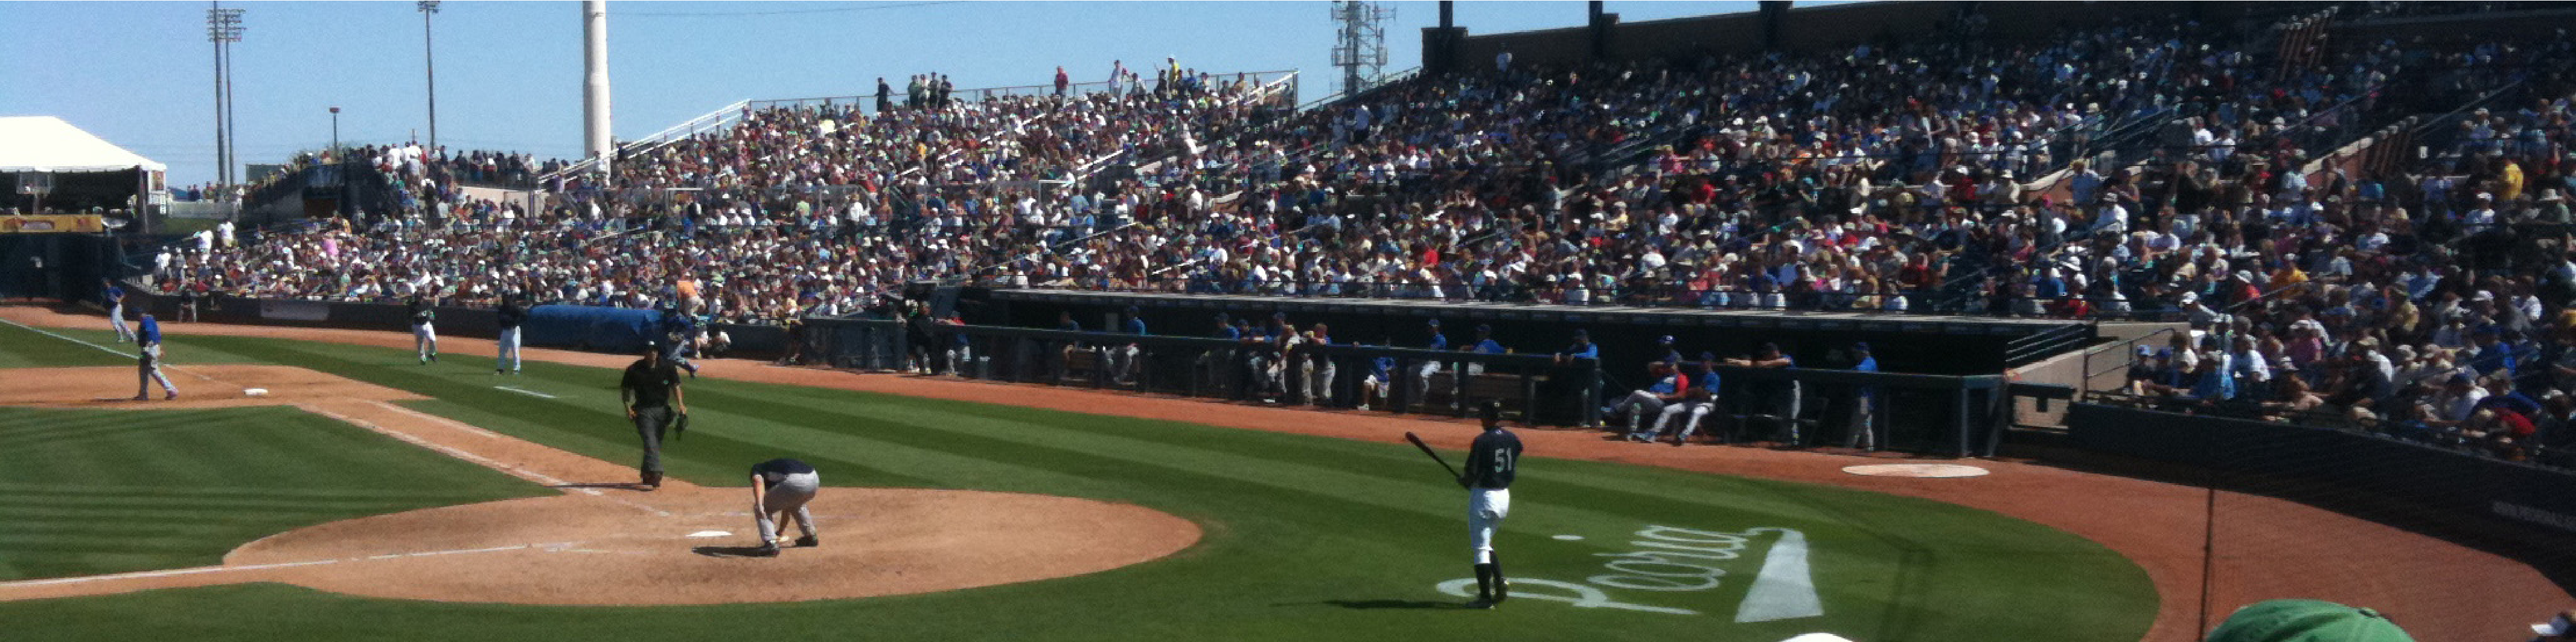
\includegraphics[width=\textwidth]{sampleteaser}
%   \caption{Seattle Mariners at Spring Training, 2010.}
%   \Description{Enjoying the baseball game from the third-base
%   seats. Ichiro Suzuki preparing to bat.}
%   \label{fig:teaser}
% \end{teaserfigure}

% \received{10 May 2025}

%%
%% This command processes the author and affiliation and title
%% information and builds the first part of the formatted document.
\maketitle

\section{Introduction}
In the educational landscape, students often struggle with inconsistent study habits, frequently resorting to cramming before exams rather than engaging in regular, spaced learning. This approach is counterproductive as it hinders deep understanding and long-term retention of information. Many existing study tools inadvertently facilitate these poor techniques by failing to provide proper motivation to students, which undermines effective learning. 

Addressing this issue is crucial because consistent study habits enable better academic performance and reinforce essential learning skills, benefiting students both academically and personally. To combat this, we have used this project as an opportunity to create a new studying platform that promotes effective learning practices, ultimately fostering sustained habits that set students up for success. 

The platform allows teachers to create quizzes for their students to take, rewarding points based on their completion and performance. These points can be redeemed for in-app rewards such as avatars, visual themes, and titles/ranks. By capping daily point earnings, the platform encourages users to return regularly and study in bursts rather than all at once, aligning with psychological findings that small, regular study sessions promote deeper learning. 

Furthermore, the architectural focus of this project ensures scalability and a smooth development process. This approach keeps our code aligned with core functionality while ensuring its capacity to grow with an increasing number of users and content. By prioritizing architecture, the project serves as a case study demonstrating the usefulness of structural design in facilitating a seamless development journey at all stages. 

This structured approach not only addresses the problem of poor study habits but also ensures that the platform is both effective and adaptable, making it accessible to a broad audience with clear and professional language.

\section{Background}


\section{Approach}


\section{Outline of Project Plan}


\section{Conclusions and Future Work}


%%
%% The next two lines define the bibliography style to be used, and
%% the bibliography file.
\bibliographystyle{ACM-Reference-Format}
\bibliography{sample-base}


%%
%% If your work has an appendix, this is the place to put it.
\appendix

\section{Division of Work}


\end{document}
\endinput
%%
%% End of file `sample-sigconf.tex'.
